\documentclass[twocolumn,a4j]{jsarticle}
\setlength{\topmargin}{-20.4cm}
\setlength{\oddsidemargin}{-10.4mm}
\setlength{\evensidemargin}{-10.4mm}
\setlength{\textwidth}{18cm}
\setlength{\textheight}{26cm}

\usepackage[top=15truemm,bottom=20truemm,left=20truemm,right=20truemm]{geometry}
\usepackage[latin1]{inputenc}
\usepackage{amsmath}
\usepackage{amsfonts}
\usepackage{amssymb}
\usepackage[dvipdfmx]{graphicx}
\usepackage[hang,small,bf]{caption}
\usepackage[subrefformat=parens]{subcaption}
\usepackage[dvipdfmx]{color}
\usepackage{listings}
\usepackage{listings,jvlisting}
\usepackage{geometry}
\usepackage{framed}
\usepackage{color}
\usepackage[dvipdfmx]{hyperref}
\usepackage{ascmac}
\usepackage{enumerate}
\usepackage{tabularx}
\usepackage{cancel}
\usepackage{scalefnt}
\usepackage{overcite}
\usepackage{otf}
\usepackage{multicol}
\usepackage[geometry]{ifsym}

\renewcommand{\figurename}{Fig.}
\renewcommand{\tablename}{Table }

\lstset{
basicstyle={\ttfamily},
identifierstyle={\small},
commentstyle={\smallitshape},
keywordstyle={\small\bfseries},
ndkeywordstyle={\small},
stringstyle={\small\ttfamily},
frame={tb},
breaklines=true,
columns=[l]{fullflexible},
xrightmargin=0zw,
xleftmargin=3zw,
numberstyle={\scriptsize},
stepnumber=1,
numbersep=1zw,
lineskip=-0.5ex
}

% キャプション後ろのダブルコロンを消す
\makeatletter
\long\def\@makecaption#1#2{%
  \vskip\abovecaptionskip
  \iftdir\sbox\@tempboxa{#1\hskip1zw#2}%
    \else\sbox\@tempboxa{#1 #2}%
  \fi
  \ifdim \wd\@tempboxa >\hsize
    \iftdir #1\hskip1zw#2\relax\par
      \else #1 #2\relax\par\fi
  \else
    \global \@minipagefalse
    \hbox to\hsize{\hfil\box\@tempboxa\hfil}%
  \fi
  \vskip\belowcaptionskip}
\makeatother

% タイトル
\makeatletter
\def\@maketitle
{
\begin{center}
{\LARGE \@title \par}
\end{center}
\begin{flushright}
{\large \@date 報告書 No.27}\\
{\large M2 \@author}
\end{flushright}
\par\vskip 1.5em
}
\makeatother

\author{来代 勝胤}
\title{令和4年度 5月 第1週 報告書}
\date{2022/5/2}

\begin{document}
\columnseprule=0.1mm
\maketitle

\section*{報告内容}
\begin{enumerate}[1.]
  \item 数値シミュレーションデータの作成
  \item 実用性評価の結果
  \item 今後の予定
\end{enumerate}

\section{数値シミュレーションデータの作成}
\subsection{シミュレーション条件}
\begin{table}[hbtp]
  \label{table:data_type}
  \caption{作成予定のシミュレーション条件}
  \centering
  \begin{tabular}{ c | c | c }
           & \textgt{粒子数密度} [-/枚] & \textgt{角速度} [deg/s] \\ \hline
    Case 1 & 100                        & 5.0                     \\ \hline
    Case 2 & 100                        & 10.0                    \\ \hline
    Case 3 & 100                        & 15.0                    \\ \hline
    Case 4 & 200                        & 5.0                     \\ \hline
    Case 5 & 200                        & 15.0                    \\ \hline
    Case 6 & 200                        & 10.0                    \\ \hline
    Case 7 & 300                        & 5.0                     \\ \hline
    Case 8 & 300                        & 10.0                    \\ \hline
    Case 9 & 300                        & 15.0                    \\ \hline
  \end{tabular}
\end{table}

\subsection{Case 1 についてのPIV結果}
\begin{figure}[htbp]
  \footnotesize
  \begin{center}
    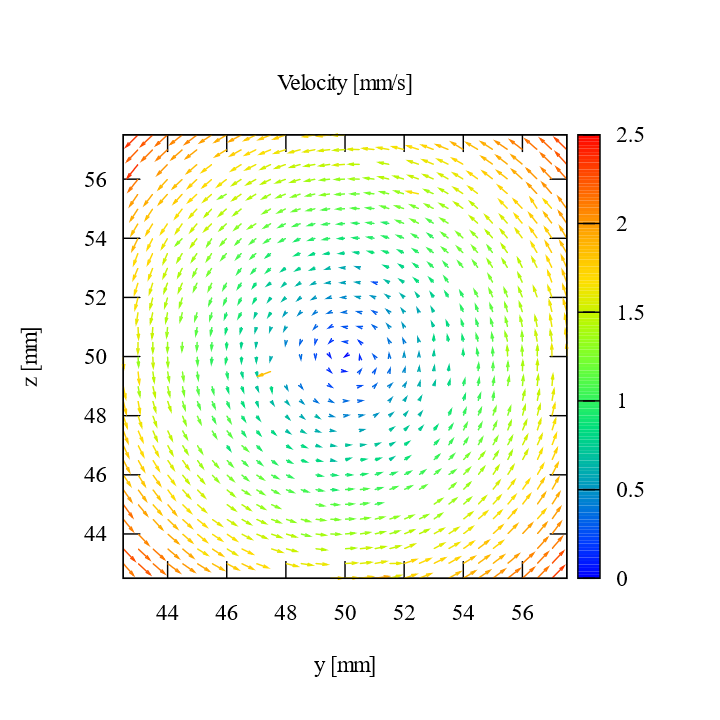
\includegraphics[width=80mm]{../images/vector_simulation.png}
    \caption{PIV result of velocity}
  \end{center}
\end{figure}

\newpage
\subsection{速度場の真値}
\begin{figure}[htbp]
  \footnotesize
  \begin{center}
    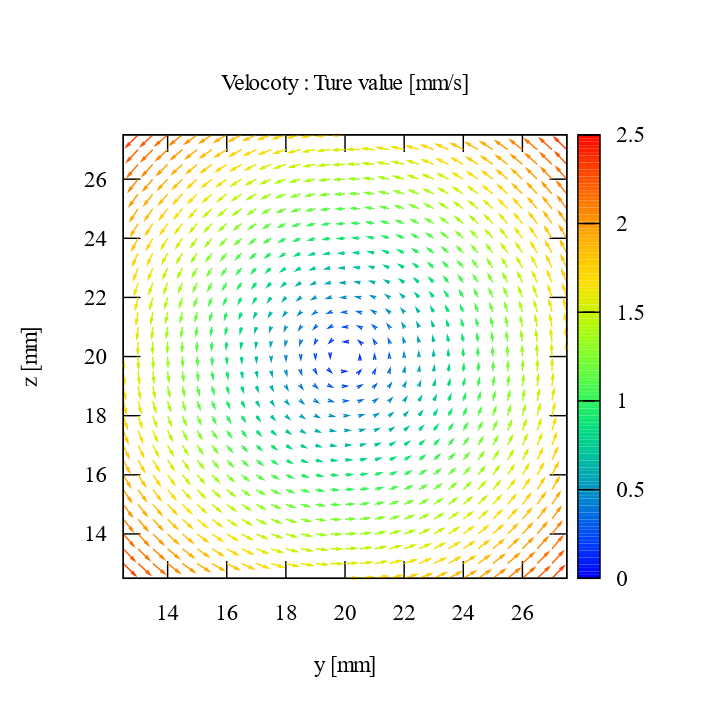
\includegraphics[width=80mm]{../images/vector_true_value.png}
    \caption{True value of velocity}
  \end{center}
\end{figure}

\section{実用性評価の結果}
\begin{table}[hbtp]
  \label{table:data_type}
  \caption{RMSEによる誤差の値と誤差率}
  \centering
  \begin{tabular}{ c | c c }
    \hline
    RMSE                & 0.083 & [mm/s] \\ \hline
    Error ratio of RMSE & 3.316 & [\%]   \\ \hline
  \end{tabular}
\end{table}

\section{来週の予定}
\begin{itemize}
  \item 日本実験力学会 登録内容 決定
  \item 三角翼の流れ場測定
  \item 粒子数密度の検討
  \item 車両モデル測定実験に向けた準備
\end{itemize}

\end{document}